\documentclass[11pt]{article}

\usepackage[a4paper,margin=2.4cm]{geometry}
\usepackage{amsmath,amssymb}
\usepackage{graphicx}
\usepackage{float}
\usepackage{adjustbox}
\usepackage{subcaption}
\usepackage{booktabs}
\usepackage{siunitx}
\usepackage{xcolor}
\usepackage{caption}
\usepackage[hidelinks]{hyperref}

\graphicspath{{figures/}}

% A per-algorithm reference: for each solver, how it works, how to use it by default, and how
% to use it at its best. Kept technical and short — a hand-over document, not a journal article.
\title{Reconstruction algorithms for MA-TIRF 3D and 2D deconvolution\\[2pt]
       \large A per-algorithm reference}
\author{Ferdinand Plesse--Costa}
\date{\today}

\begin{document}
\maketitle

\begin{abstract}
\noindent A reference for the six reconstruction algorithms in \texttt{matirf\_python\_plus} ---
Adam, PPXA, ADMM, PnP-HQS, ADMM-PnP and MCMC --- on the MA-TIRF 3D depth-reconstruction problem
and, as a well-posed companion, on 2D deconvolution. MA-TIRF is severely ill-posed: the forward
operator determines only two to three of ${\sim}50$ depth directions per column, so the prior ---
not the optimiser --- sets the ceiling. Each algorithm gets one chapter: how it works, its
\emph{standard} (default) use, its \emph{optimal} use (the best measured parameters), and the
intrinsic limit no parameter moves. The short preamble fixes the shared facts every chapter
rests on; a comparison table and a one-page decision guide close the document.
\end{abstract}

\tableofcontents
\bigskip

\section{The shared ground}
\label{sec:preamble}

Everything in the algorithm chapters rests on four facts. They are stated once here; the full
derivations are in \texttt{matirf\_python\_plus/docs/algorithms/00\_foundation.md}.

\paragraph{1. The forward model.}
Both problems are linear with a non-negativity constraint,
\begin{equation}
  g = Hf + n, \qquad f \ge 0, \qquad \max g = 1,
  \label{eq:forward}
\end{equation}
with $f$ the unknown object, $H$ the known operator, $n$ the detector noise and $g$ the
peak-normalised measurement. For MA-TIRF, $H$ acts independently in each lateral pixel: it mixes
the $n_z$ depth planes of a column into the measured angle values, so it is one small
$n_\theta \times n_z$ matrix applied to every column. For deconvolution $H$ is a convolution with
a known PSF.

\paragraph{2. The one fact that governs everything --- the spectrum of $H$.}
The per-column MA-TIRF matrix (13 angles, $n_z=50$ over \SIrange{0}{300}{\nano\meter}, physical
operator) has singular values that collapse by orders of magnitude:
\begin{center}
\begin{tabular}{lccccc}
\toprule
 & $s_1$ & $s_2$ & $s_3$ & $s_4$ & $s_5\dots$ \\
\midrule
$s$   & 38.9 & 6.02 & 0.562 & 0.033 & $<10^{-3}$ \\
$s^2$ & $1.5\times10^{3}$ & 36 & 0.32 & $1.1\times10^{-3}$ & \\
\bottomrule
\end{tabular}
\end{center}
Only two to three depth directions per column are determined by the data; the other ${\sim}47$ of
50 lie in the numerical null space of $H$. \textbf{The prior --- not the optimiser --- decides
those ${\sim}47$ directions.} This single fact drives every result: the ceiling on a
reconstruction is set by the prior, and the universal failure mode is \emph{depth collapse} (the
object slides or flattens in $z$, exactly where the data are blind). For deconvolution the
spectrum is continuous and decays smoothly, so ranges tied to the discrete $s_i^2$ do not
transfer as-is between the two problems.

\paragraph{3. The scale of the unknown.}
Along the best-determined direction $g_1 = s_1 f_1$ with $\max g = 1$, so $f$ peaks at
${\approx}1/s_1 \approx 0.02$ on MA-TIRF (and ${\approx}1$ on deconvolution). \textbf{Any
parameter in units of $f$} --- a step size, a proposal noise, a sparsity threshold, a denoiser
level --- \textbf{must be compared to ${\sim}0.02$, not to $1$}; a default tuned for a photograph
is ${\approx}s_1 \approx 40\times$ off. This is the most common way a method that works elsewhere
silently fails here.

\paragraph{4. Two estimators, one objective.}
The MAP solvers (Adam, PPXA, ADMM, PnP-HQS, ADMM-PnP) minimise an energy
\begin{equation}
  L(f) = (1-\lambda)\, D(Hf,g) + \lambda\,\kappa\, R(f), \qquad f \ge 0,\ \lambda \in [0,1],
  \label{eq:objective}
\end{equation}
with $D$ the per-pixel negative log-likelihood ($\lVert Hf-g\rVert^2/(2 b n_g)$ for Gaussian
noise of variance $b$), which carries the noise level and sits at ${\approx}\tfrac12$ at the truth
(a $\chi^2$ anchor, $\texttt{chi2\_ratio}=2D$). $R$ is the regulariser; the scalar
$\kappa = 1/R(f_{\text{init}})$ rescales it onto $D$'s scale so that $\lambda$ reads as a
regularisation \emph{share}. The MMSE solver (MCMC) returns the posterior mean by sampling.
ADMM, PnP and ADMM-PnP hard-wire their prior (a soft threshold, or a denoiser) and do not use
$R$, $\lambda$ or $\kappa$.

\paragraph{Metrics.}
Reconstructions with a ground truth are scored by \textbf{NMSE} (overall error, 0 perfect),
\textbf{PSNR} (the same in dB, monotone in NMSE), \textbf{Depth Error (nm)} (mean axial
mislocalisation --- \emph{the} MA-TIRF question) and \textbf{Stack Recovery} (fraction of
\SI{\ge30}{\nano\meter} pairs resolved); 2D deconvolution adds \textbf{SSIM} (unreliable on the
anisotropic MA-TIRF volume, so deconv-only). Without a truth --- the real \texttt{esoubies} data
--- the only quality number is \texttt{chi2\_ratio} (data fit, ${\approx}1$ good). Each run also
records runtime, peak memory and status (ok / rejected / out-of-memory / timeout): a solver that
runs out of memory on a real stack is disqualified by that alone.

\paragraph{The benchmark behind the numbers.}
Every measured value below comes from one curated campaign
(\texttt{matirf\_python\_plus/benchmarks/}, Sec.~\ref{sec:repro}) on \textbf{three primitive
structures} --- point-like \texttt{vesicles}, filaments \texttt{fibres} and a continuous membrane
\texttt{cell} --- each across three noise levels $\{0,\,0.02,\,0.05\}$, plus the 2D companion
\texttt{img\_001} and the real \texttt{esoubies} measurement (reconstructed by every solver). For
each algorithm the campaign runs its \emph{standard} (default) configuration, its \emph{best-known}
one, and --- for the denoiser-based methods --- a sweep of denoisers, so the ``standard vs
optimal'' and ``which denoiser'' tables are measured per structure, not asserted. Testing three
structures is deliberate: the best prior, and the best denoiser, depend on the object.

\section{Adam --- general MAP minimiser}
\label{sec:adam}

\paragraph{How it works.}
Adam minimises the objective~\eqref{eq:objective} by gradient descent with a per-coordinate
adaptive step, positivity by clamping, a learning rate halved whenever the loss rises, and a
small-change stop:
\begin{quote}\small
$f \leftarrow f_0$ (the ridge $s_2^2$ start);\quad
repeat: $g_k \leftarrow \nabla L(f)$;\ $f \leftarrow f - \text{lr}\cdot \hat m/(\sqrt{\hat v}+\varepsilon)$;\
$f \leftarrow \max(f,0)$;\ every $K$ steps halve lr if the loss rose, stop if it barely moved.
\end{quote}
Because $\lvert \hat m/\sqrt{\hat v}\rvert \approx 1$, each voxel moves by about \texttt{lr} per
iteration \emph{whatever the gradient} --- so \texttt{lr} is a displacement in the units of $f$
(${\sim}0.02$), not a gradient scaling. $L$ is convex, so with a prior that weighs the minimiser
is unique and Adam reaches it; the reconstruction is then only as good as the analytic prior $R$.

\paragraph{Parameters.}
The only axes that move the \emph{solution} are the prior \texttt{reg} and its share $\lambda$.
We compare two priors: \textbf{L1} (sparsity --- few bright voxels) and \textbf{Tikhonov} (the
L2 of the gradient --- smoothness). Tikhonov is a degree-2 prior, so at $f\approx0.02$ it is
${\sim}50\times$ weaker than a degree-1 prior for the same nominal $\lambda$ and over-smooths once
it bites. Everything else is a convergence knob, fixed for the whole campaign: \texttt{lr}$=0.1$
(large enough to move; the scheduler halves it on overshoot), \texttt{init}$=$ridge with weight
$\lambda_{rr}=s_2^2=36.24$ (never the adjoint start, ${\sim}850\times$ too large at MA-TIRF
scale), \texttt{max\_iter}$=5000$ and \texttt{EPS}$=10^{-8}$ so the plateau stop --- not the
budget --- ends the run.

\paragraph{Standard use.}
The smooth prior at a moderate share, $\texttt{reg}=\text{Tikhonov}$, $\lambda=0.1$. It is a safe
default that never empties the image, but it over-smooths depth --- rarely the best prior on the
sparse structures, though closer to competitive on the continuous membrane.

\paragraph{Optimal use.}
Match the prior to the object and raise it with the noise. On the sparse structures (filaments,
vesicles) the sparsity prior L1 has a clear optimum, while the smooth Tikhonov prior only
over-smooths --- its NMSE stays high and flat:
\IfFileExists{tables/adam_shape.tex}{\begin{center}\begin{minipage}{\linewidth}\centering
\captionof{table}{Adam --- prior shape at the reference structure (noise 0.02): NMSE and depth error versus lambda for the sparse (L1) and smooth (Tikhonov) priors.}
\begin{adjustbox}{max width=\linewidth}
\begin{tabular}{llll}
\toprule
prior & lambda & NMSE & depth err (nm) \\
\midrule
l1 & 0.05 & 0.478 & 48 \\
l1 & 0.1 & 0.507 & 54 \\
tikhonov & 0.05 & 0.405 & 66 \\
tikhonov & 0.2 & 0.459 & 80 \\
tikhonov & 0.3 & 0.483 & 87 \\
tikhonov & 0.5 & 0.527 & 97 \\
\bottomrule
\end{tabular}\end{adjustbox}\end{minipage}\end{center}
}%
  {\emph{[pending the run — \texttt{python -m benchmarks analyze}]}}

\noindent L1 minimises around $\lambda \approx 0.2$--$0.3$; Tikhonov, being smooth and degree-2,
cannot localise a filament network and trails it throughout. The prior winner may itself shift with
the object (the smooth prior is less penalised on a continuous membrane) --- the measured
standard-vs-optimal figures, per structure:
\IfFileExists{tables/algo_adam.tex}{\begin{center}\begin{minipage}{\linewidth}\centering
\captionof{table}{ADAM on MA-TIRF --- reconstruction metrics per ground truth and noise level.}
\begin{adjustbox}{max width=\linewidth}
\begin{tabular}{llllllll}
\toprule
dataset & noise & params & NMSE & PSNR & Depth Error (nm) & Stack Recovery & chi2\_ratio \\
\midrule
cell & 0 & reg=tikhonov, lambda=0.1 & 0.72 & 15.2 & 60 & 0 & 0.00507 \\
cell & 0 & reg=none, lambda=0 & 0.476 & 17.0 & 21 & 0 & 1.17e-06 \\
fibres & 0 & reg=tikhonov, lambda=0.1 & 0.321 & 29.0 & 58 & 0.241 & 0.0298 \\
fibres & 0 & reg=none, lambda=0 & 0.0812 & 34.9 & 14 & 0 & 1.59e-05 \\
vesicles & 0 & reg=tikhonov, lambda=0.1 & 0.481 & 29.3 & 69 & 0.5 & 0.048 \\
vesicles & 0 & reg=none, lambda=0 & 0.0697 & 37.7 & 2 & 0 & 1.1e-05 \\
cell & 0.02 & reg=tikhonov, lambda=0.1 & 0.534 & 16.5 & 26 & 0.0758 & 0.653 \\
cell & 0.02 & reg=l1, lambda=0.2 & 0.277 & 19.4 & 16 & 0 & 0.591 \\
fibres & 0.02 & reg=tikhonov, lambda=0.1 & 0.429 & 27.7 & 72 & 0.0431 & 0.433 \\
fibres & 0.02 & reg=tikhonov, lambda=0.05 & 0.405 & 28.0 & 66 & 0.0862 & 0.415 \\
vesicles & 0.02 & reg=tikhonov, lambda=0.1 & 0.552 & 28.7 & 69 & 0 & 0.423 \\
cell & 0.05 & reg=tikhonov, lambda=0.1 & 0.584 & 16.1 & 30 & 0.0606 & 0.615 \\
cell & 0.05 & reg=l1, lambda=0.2 & 0.487 & 16.9 & 22 & 0 & 0.596 \\
fibres & 0.05 & reg=tikhonov, lambda=0.1 & 0.679 & 25.7 & 115 & 0.0431 & 0.411 \\
vesicles & 0.05 & reg=tikhonov, lambda=0.1 & 0.787 & 27.1 & 146 & 0 & 0.391 \\
esoubies & native & reg=l1, lambda=0.2 & — & — & — & — & 18.9 \\
\bottomrule
\end{tabular}\end{adjustbox}\end{minipage}\end{center}
\begin{center}\begin{minipage}{\linewidth}\centering
\captionof{table}{ADAM on deconvolution --- reconstruction metrics per noise level.}
\begin{adjustbox}{max width=\linewidth}
\begin{tabular}{lllllll}
\toprule
dataset & noise & params & NMSE & PSNR & SSIM & chi2\_ratio \\
\midrule
img\_001 & 0 & reg=tikhonov, lambda=0.1 & 0.195 & 14.1 & 0.302 & 0.021 \\
img\_001 & 0 & reg=none, lambda=0 & 0.0191 & 24.4 & 0.694 & 1.96e-07 \\
img\_001 & 0.02 & reg=tikhonov, lambda=0.1 & 0.0293 & 22.6 & 0.576 & 1.09 \\
img\_001 & 0.05 & reg=tikhonov, lambda=0.1 & 0.0371 & 21.5 & 0.511 & 1.09 \\
\bottomrule
\end{tabular}\end{adjustbox}\end{minipage}\end{center}
}{}

\IfFileExists{figures/matirf_fibres_ADAM_noise002.png}{%
\begin{figure}[H]\centering
  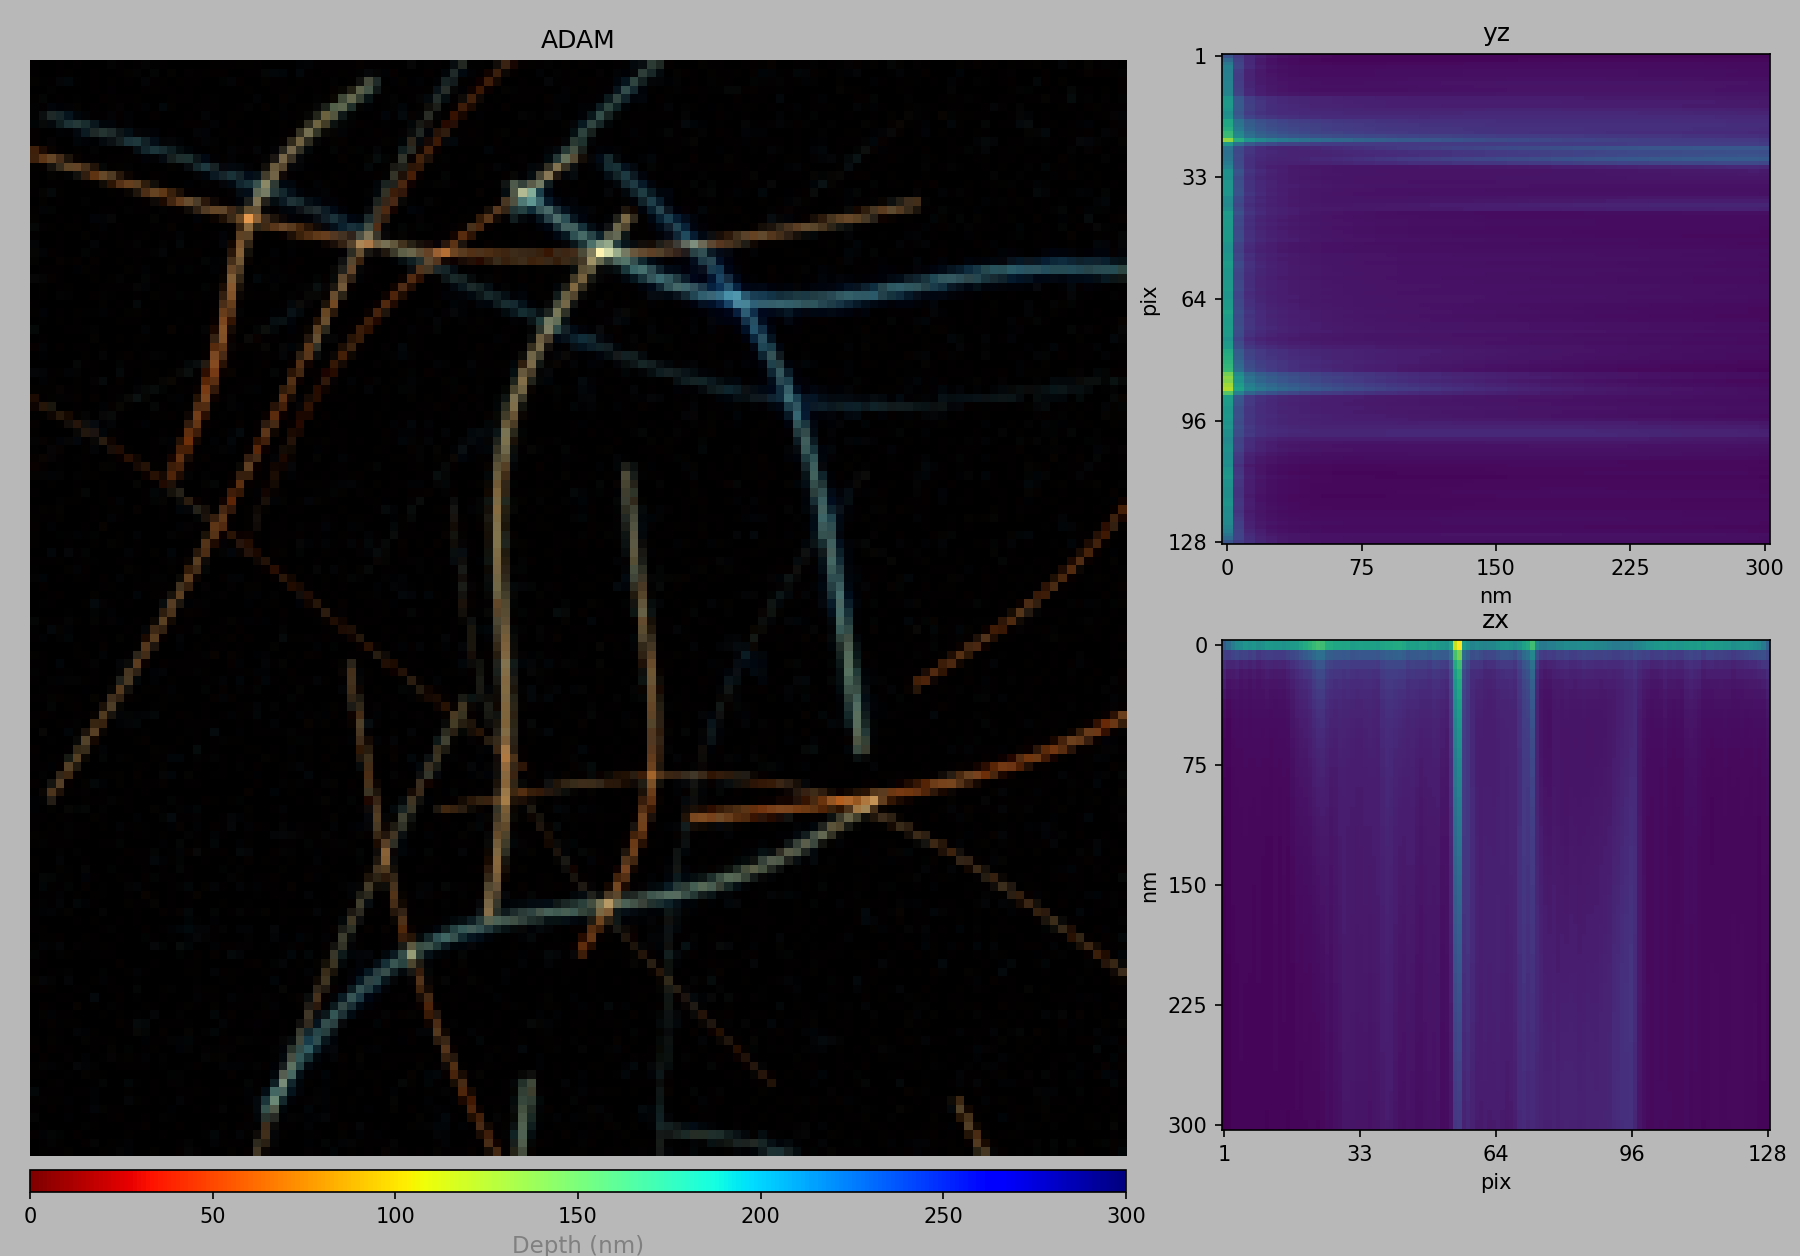
\includegraphics[width=.7\linewidth]{matirf_fibres_ADAM_noise002}
  \caption{Adam's best reconstruction of \texttt{fibres} at noise 0.02 (depth map + $yz/zx$
  profiles).}
\end{figure}}{}

\paragraph{When it works, when it fails.}
Adam has no failure of its own on a well-posed problem: it minimises the energy exactly. On
MA-TIRF the quality is decided entirely by $R$ and $\lambda$, and none of the analytic priors
models a cell's depth structure the way a learned denoiser does --- \emph{its ceiling is the
ceiling of hand-built priors}. The failure modes are at the ends of $\lambda$: $\lambda\to0$ is
non-negative least squares (noisy / depth-collapsed), $\lambda\to1$ drops the data (empty or
flat). Adam is the right \emph{engine} and, on MA-TIRF, the wrong \emph{prior}: the gain is in
the regulariser, not the optimiser.

\section{PPXA --- proximal splitting twin of Adam}
\label{sec:ppxa}

\paragraph{How it works.}
PPXA minimises the \emph{same} objective~\eqref{eq:objective} as Adam, but by evaluating each
term's proximal operator in parallel, averaging, and over-relaxing:
\begin{quote}
$p_1 \leftarrow (I+\gamma H^{\!\top}\!H)^{-1}(u_1+\gamma H^{\!\top} g)$ \hfill\textit{(data prox: pull toward $g$)}\\
$p_2 \leftarrow \mathrm{prox}_{\gamma\lambda R}(u_2)$ \hfill\textit{(prior prox)}\\
$p_3 \leftarrow \max(u_3,0)$ \hfill\textit{(positivity prox)}\\
$\bar p \leftarrow \tfrac13(p_1+p_2+p_3)$ \hfill\textit{(average)}\\
$u_i \leftarrow u_i + \rho_{\mathrm{rel}}(2\bar p - f - p_i)$;\quad $f \leftarrow f + \rho_{\mathrm{rel}}(\bar p - f)$ \hfill\textit{(over-relax)}
\end{quote}
\noindent where $\gamma$ is the prox step (gain $\gamma s_i^2$ per singular direction), $u_1,u_2,u_3$
the auxiliary variables, $R$ the regulariser at share $\lambda$, and $\rho_{\mathrm{rel}}\in(0,2)$
the relaxation. Minimising the same convex $L$, it reaches the \emph{same image} as Adam.

\paragraph{Key parameters.}
The same solution axes as Adam (\texttt{reg}, $\lambda$); its own knobs set speed only, provided the
proxes are exact: $\gamma\in[1/s_1^2,1/s_2^2]$ (out of range it can stall) and
$\rho_{\mathrm{rel}}=1.5$.

\paragraph{Results.}
Run identically to Adam. The campaign confirms the framework claim --- \emph{Adam and PPXA return
the same image} on the shared L1 objective (reference structure, noise 0.02):
\IfFileExists{tables/algo_ppxa.tex}{\paragraph{matirf}
\begin{center}\begin{adjustbox}{max width=\linewidth}
\begin{tabular}{lllllllll}
\toprule
use & dataset & noise & params & NMSE & PSNR & Depth Error (nm) & Stack Recovery & chi2\_ratio \\
\midrule
optimal & esoubies & native & reg=l1, lambda=0.2 & — & — & — & — & 18.8 \\
optimal & fibres & 0.02 & reg=l1, lambda=0.2 & 0.855 & 24.7 & 73 & 0 & 0.446 \\
\bottomrule
\end{tabular}\end{adjustbox}\end{center}
}{}

\paragraph{Limit.}
PPXA shares Adam's ceiling (only as good as the analytic prior) and adds two costs: it needs
\emph{proximable} priors (Adam takes any differentiable one), and its splitting is markedly slower
here (median runtime several times Adam's).

\section{ADMM --- sparsity by soft thresholding}
\label{sec:admm}

\paragraph{How it works.}
ADMM is the MAP estimator for a \emph{sparse}, non-negative object under Gaussian noise: its
prior is hard-wired ($\ell_1$ + positivity), so it ignores $R$, $\lambda$, $\kappa$. It alternates
a data step, a soft threshold and a dual update:
\begin{quote}\small
$t = \kappa\, \max(g)/s_1$ (threshold);\quad
$u \leftarrow (H^{\!\top}\!H+\mu I)^{-1}(H^{\!\top} g + \mu(f-\eta))$;\quad
$f \leftarrow \max(u+\eta-t,\,0)$;\quad $\eta \leftarrow \eta + \mu(u-f)$.
\end{quote}
The Laplacian prior $\exp(-\tau\lVert f\rVert_1)$ says ``most voxels are ${\approx}0$, a few are
bright'' --- the right model for point-like / filamentary structures, the wrong one for a
continuous membrane.

\paragraph{Parameters.}
Two knobs move the solution, and awkwardly. The threshold ratio $\kappa$ (\texttt{threshold\_ratio})
sets the sparsity, but its useful band cannot be predicted a priori --- the data step spreads the
object across the ${\sim}47$ null-space directions, so every voxel of the ridge estimate is small
and a diffuse truth can be emptied by a modest $\kappa$. The penalty $\mu$ carries \emph{three}
coupled roles at once (data-step ridge, prior weight $\tau=\mu\kappa\max(g)/s_1$, and dual step),
and the dual step caps it: $\mu > 1.618$ oscillates or diverges (measured: $\mu=2.5\to$ NaN).
\texttt{iter}$=200$ is a generous budget (the default 20 is under-iterated).

\paragraph{Standard use.}
$\kappa=0.1$, $\mu=0.5$ ($\approx s_3^2$, inside the stable band). On a concentrated object at
low noise this is already close to the best ADMM can do.

\paragraph{Optimal use.}
Sweep $\kappa$ log-spaced (here $\kappa\in\{0.1,\,0.01\}$) and raise it with the noise; keep
$\mu \in [s_3^2,\,1.6] = [0.3,\,1.6]$. The measured standard-vs-optimal figures:
\IfFileExists{tables/algo_admm.tex}{\paragraph{matirf}
\begin{center}\begin{adjustbox}{max width=\linewidth}
\begin{tabular}{lllllllll}
\toprule
use & dataset & noise & params & NMSE & PSNR & Depth Error (nm) & Stack Recovery & chi2\_ratio \\
\midrule
standard / optimal & cell & 0 & kappa=0.1, mu=0.5 & 0.0318 & 28.8 & 4 & 0.636 & 5.2e-08 \\
standard / optimal & cell & 0.02 & kappa=0.1, mu=0.5 & 0.619 & 15.9 & 41 & 0.152 & 0.604 \\
standard / optimal & cell & 0.05 & kappa=0.1, mu=0.5 & 0.899 & 14.3 & 68 & 0.0758 & 0.589 \\
optimal & esoubies & native & kappa=0.1, mu=0.5 & — & — & — & — & 19.2 \\
standard & fibres & 0 & kappa=0.1, mu=0.5 & 0.251 & 30.1 & 15 & 0.336 & 0.000278 \\
optimal & fibres & 0 & kappa=0.01, mu=0.5 & 0.0406 & 38.0 & 10 & 0.966 & 4.86e-06 \\
standard / optimal & fibres & 0.02 & kappa=0.1, mu=0.5 & 0.882 & 24.6 & 64 & 0.0517 & 0.436 \\
standard / optimal & fibres & 0.05 & kappa=0.1, mu=0.5 & 0.973 & 24.2 & 95 & 0.0172 & 0.411 \\
standard & vesicles & 0 & kappa=0.1, mu=0.5 & 0.142 & 34.6 & 8 & 0 & 0.00024 \\
optimal & vesicles & 0 & kappa=0.01, mu=0.5 & 0.021 & 42.9 & 8 & 1 & 5.3e-06 \\
standard / optimal & vesicles & 0.02 & kappa=0.1, mu=0.5 & 0.848 & 26.8 & 66 & 0 & 0.413 \\
standard / optimal & vesicles & 0.05 & kappa=0.1, mu=0.5 & 0.974 & 26.2 & 94 & 0 & 0.39 \\
\bottomrule
\end{tabular}\end{adjustbox}\end{center}
}%
  {\emph{[pending the run]}}

\IfFileExists{figures/matirf_vesicles_ADMM_noise00.png}{%
\begin{figure}[H]\centering
  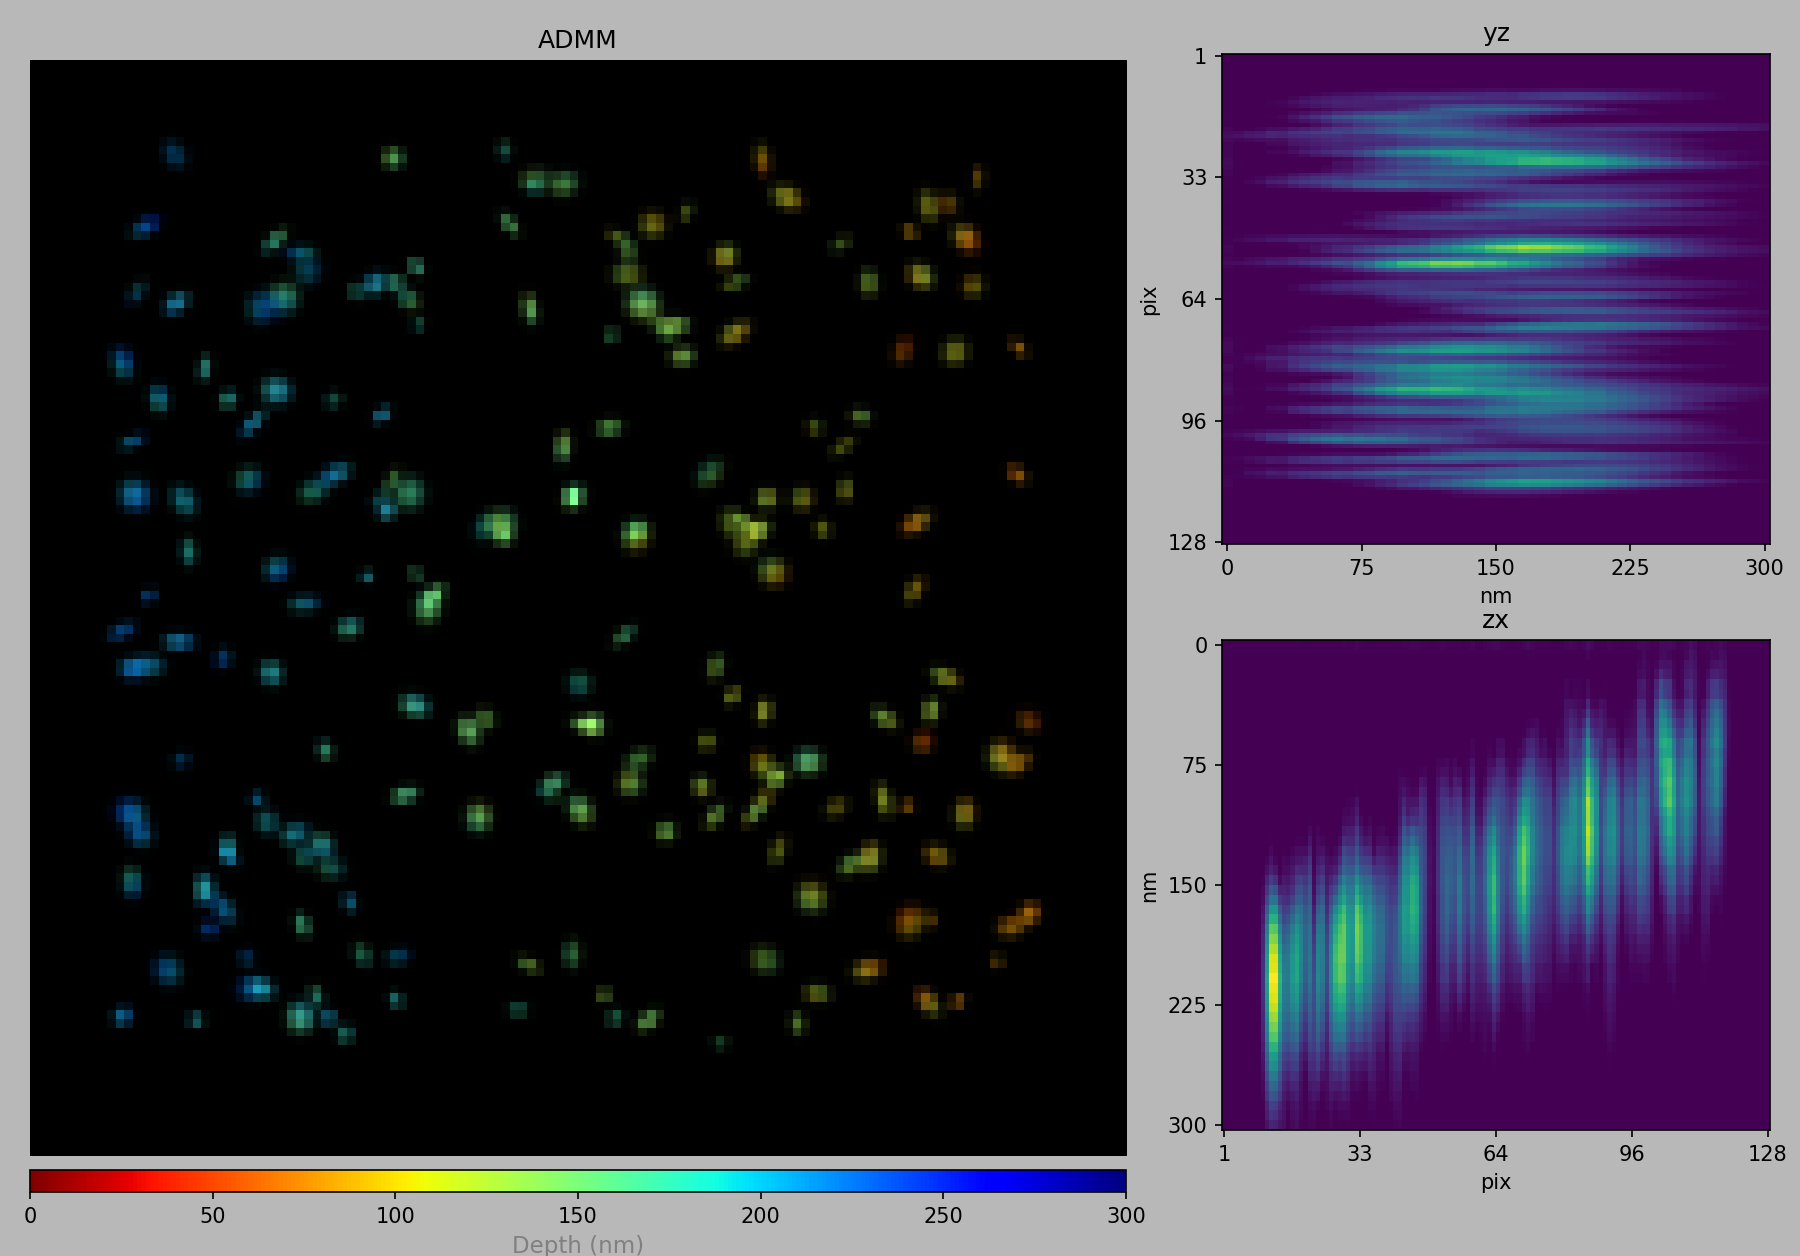
\includegraphics[width=.7\linewidth]{matirf_vesicles_ADMM_noise00}
  \caption{ADMM on \texttt{vesicles} at zero noise --- where the sparsity prior localises the
  point-like structure well.}
\end{figure}}{}

\paragraph{When it works, when it fails.}
ADMM's wall is its prior. On a diffuse or continuous object $\ell_1$ is the wrong model, so there
is little-to-no useful $\kappa$ band: $\kappa$ too large empties the image (the dominant failure,
and it arrives early), $\kappa\approx0$ is noisy and lets \texttt{iter} become an accidental
regulariser. Concentrated truths (vesicles, filaments) have a band, but a narrow one. Use ADMM
for sparse objects at low noise; do not expect it to reconstruct a membrane.

\section{PnP-HQS --- a denoiser as the prior, on a schedule}
\label{sec:pnp}

\paragraph{How it works.}
Plug-and-Play half-quadratic splitting replaces the prior's proximal operator by a \emph{denoiser}
$D_\sigma$, over a short coarse-to-fine annealing schedule (not to convergence):
\begin{quote}
$z \leftarrow f_0$ \hfill\textit{(start: the ridge $s_2^2$ estimate)}\\
\textbf{for} $k = 1 \dots \texttt{iter}$, with $\sigma_k\!\downarrow$ and $\alpha_k\!\uparrow$:\\
\hspace{1.2em}$f \leftarrow (H^{\!\top}\!H+\alpha_k I)^{-1}(H^{\!\top} g + \alpha_k z)$ \hfill\textit{(data step: fit $g$, pulled toward $z$)}\\
\hspace{1.2em}$z \leftarrow \tfrac{\text{peak}}{255}\,D_{\sigma_k}\!\big(255\,f/\text{peak}\big)$ \hfill\textit{(denoise at level $\sigma_k$, scale-free)}
\end{quote}
\noindent where $D_\sigma$ is the denoiser, $\sigma_k$ its level (annealed from $\sigma$ down to the
measurement's noise), $\alpha_k$ the data-coupling weight (annealed \emph{up} to
$\lambda_{kz}=\alpha_{\text{final}}$), and $\text{peak}$ the start's peak. Since $s_i^2\ll\alpha$
keeps the denoised $z$, the ${\sim}47$ null-space directions are the denoiser's --- it has no dual
variable, so the schedule alone drives the prior in.

\paragraph{Key parameters.}
The denoiser and its level $\sigma$; the final data weight $\lambda_{kz}=\alpha_{\text{final}}$ is a
\textbf{threshold on the eigenvalues} $s_i^2$: at $\lambda_{kz}\approx12$ only $s_1,s_2$ follow the
data and the whole null space goes to the prior --- what an ill-posed problem needs. (The DPIR
default $\lambda_{kz}=0.23$, tuned for deconvolution, under-uses the prior and is data-starved
here.) \texttt{iter} is a real lever too --- more schedule steps keep improving, past the usual
$[8,30]$.

\paragraph{Results.}
With $\lambda_{kz}\approx12$, \texttt{iter}${\approx}40$ and the right denoiser, PnP reconstructs
well; the best denoiser depends on the object (Table~\ref{tab:denoisers}) --- Gaussian on the
filament network, TV~Bregman on the membrane under noise, DCT competitive.
\IfFileExists{tables/gallery_pnp.tex}{\begin{figure}[H]\centering
\begin{subfigure}{0.56\linewidth}\centering
\IfFileExists{figures/matirf_vesicles_PNP_noise002.png}{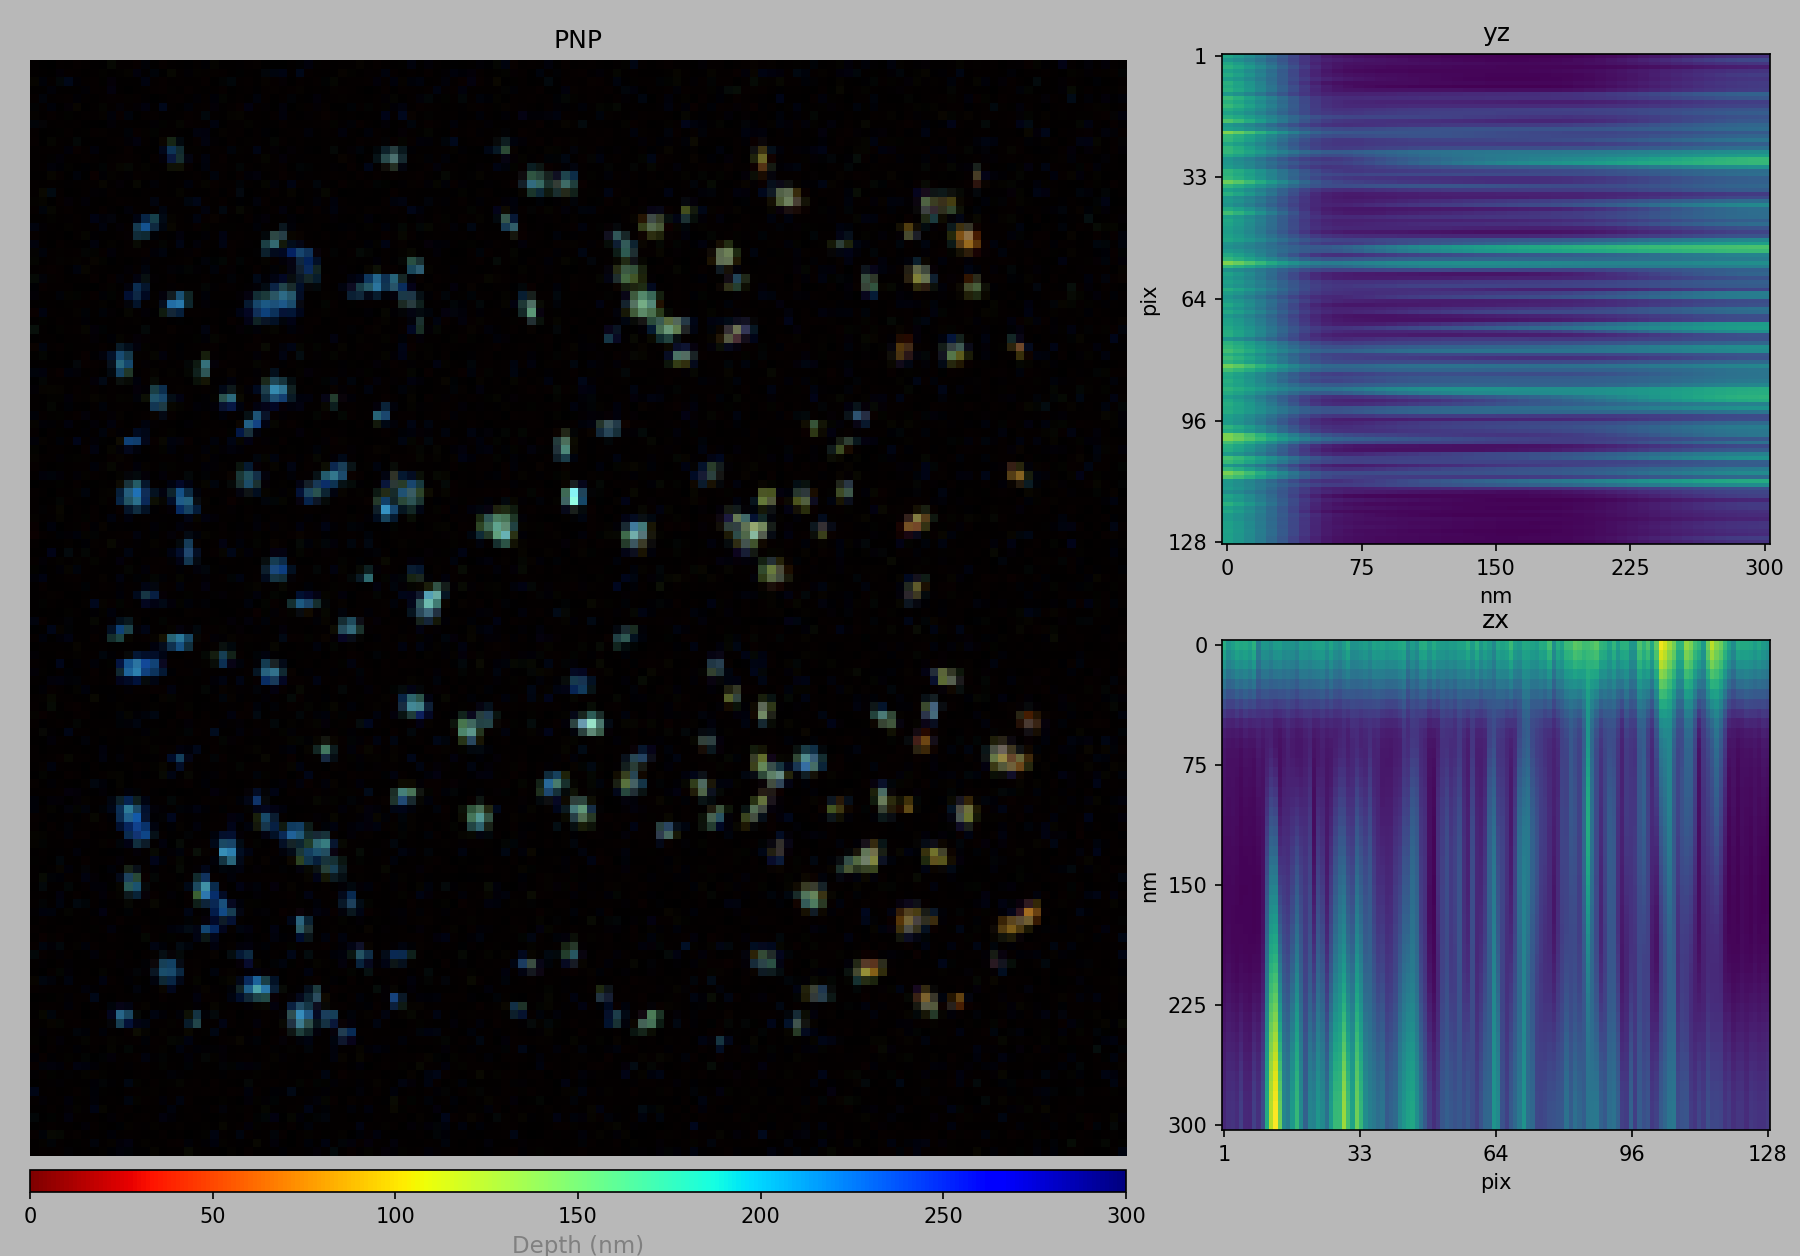
\includegraphics[width=\linewidth]{matirf_vesicles_PNP_noise002}}{}
\caption*{\footnotesize\texttt{vesicles} --- denoiser=Gaussian, sigma=25, lambda\_kz=12, iter=40 (NMSE 0.522)}
\end{subfigure}\par\smallskip
\begin{subfigure}{0.56\linewidth}\centering
\IfFileExists{figures/matirf_fibres_PNP_noise002.png}{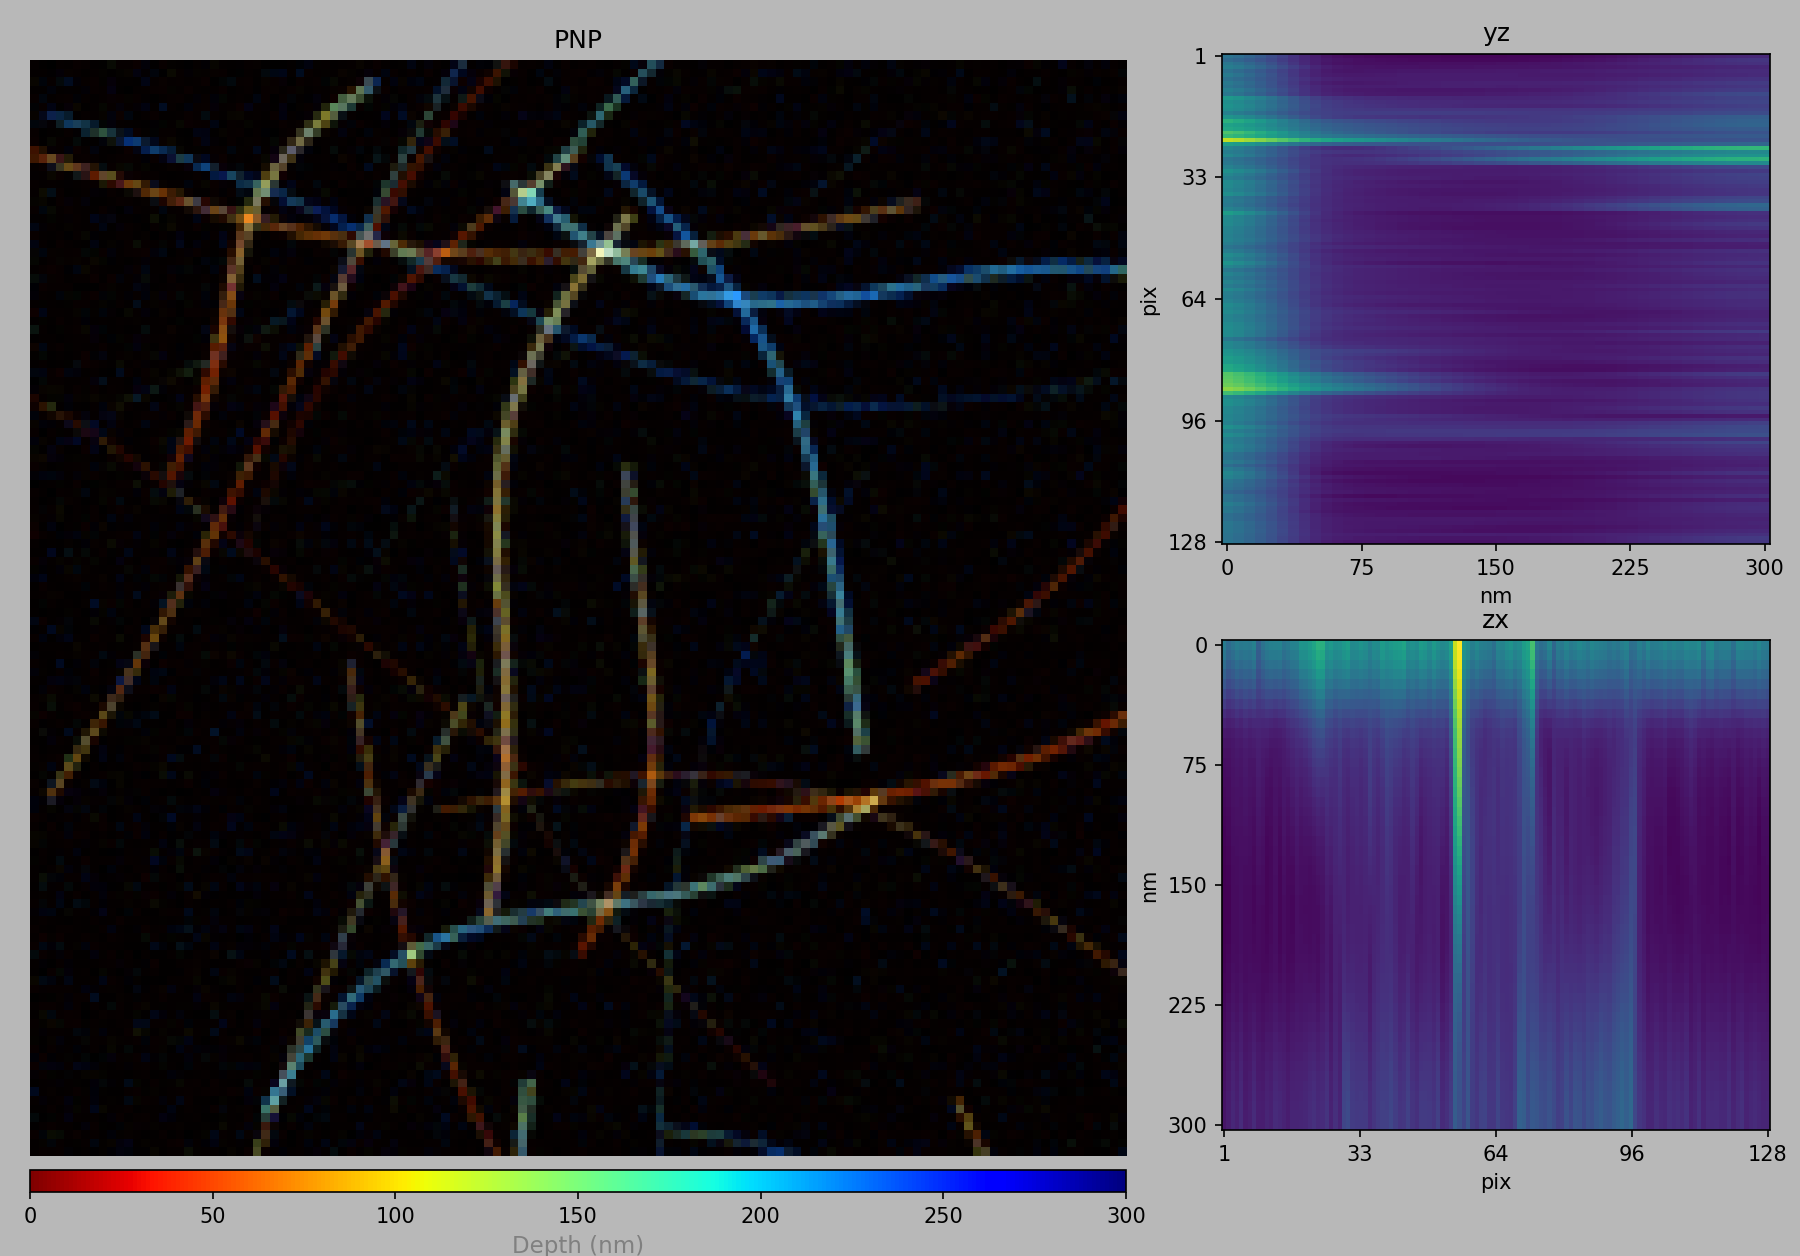
\includegraphics[width=\linewidth]{matirf_fibres_PNP_noise002}}{}
\caption*{\footnotesize\texttt{fibres} --- denoiser=Gaussian, sigma=25, lambda\_kz=12, iter=40 (NMSE 0.385)}
\end{subfigure}\par\smallskip
\begin{subfigure}{0.56\linewidth}\centering
\IfFileExists{figures/matirf_cell_PNP_noise002.png}{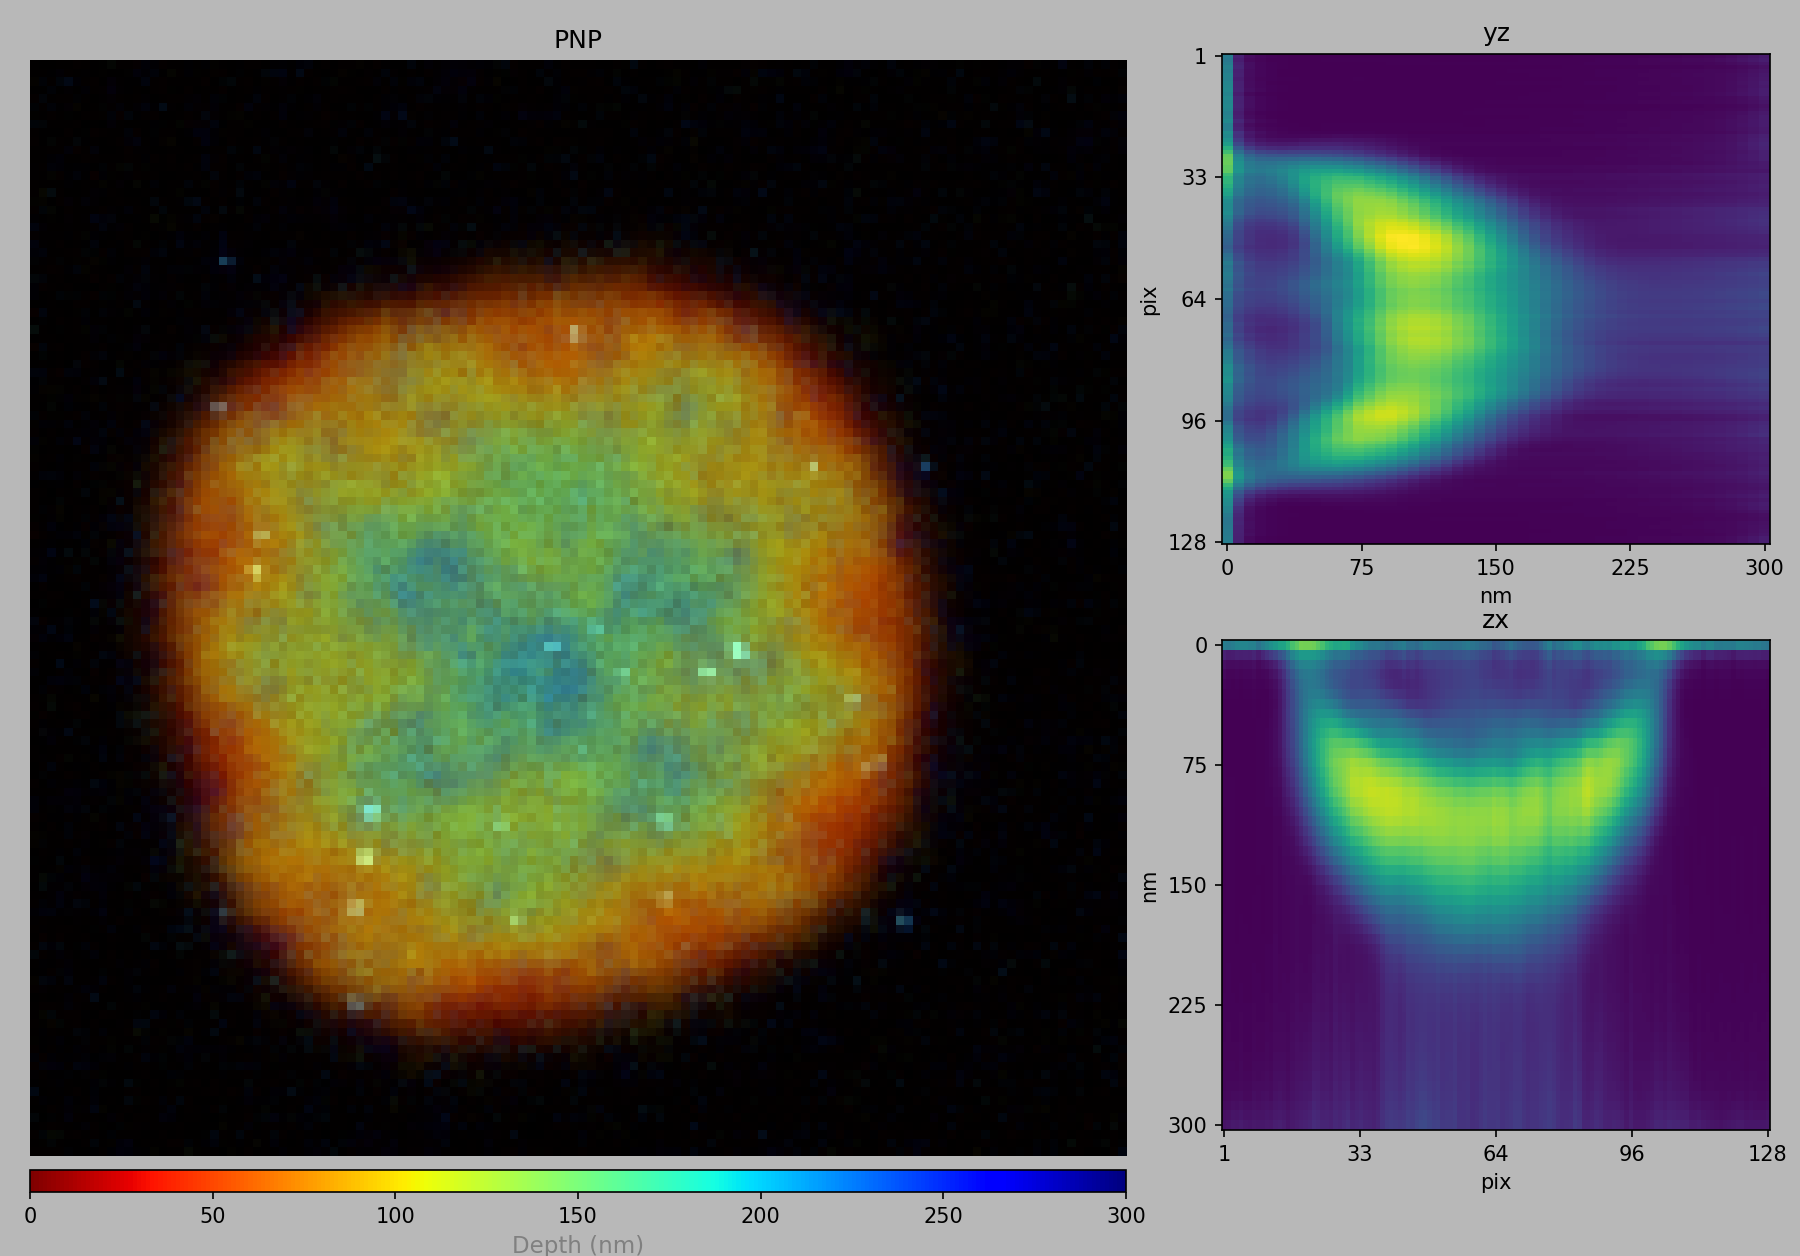
\includegraphics[width=\linewidth]{matirf_cell_PNP_noise002}}{}
\caption*{\footnotesize\texttt{cell} --- denoiser=TV Bregman, sigma=40, lambda\_kz=12, iter=40 (NMSE 0.262)}
\end{subfigure}\par\smallskip
\caption{\textbf{PNP} --- best reconstruction on each structure at noise 0.02 (depth map + $yz/zx$ profiles; the parameters under each panel reproduce it).}
\end{figure}
}{}

\paragraph{Limit.}
Two intrinsic limits. \emph{Scale}: a denoiser transfers only if fed at the scale it was built for
--- the $255\,f/\text{peak}$ bridge is what makes even DCT usable on MA-TIRF (it is \emph{not}
categorically broken, contrary to the naive-scale belief). \emph{Cost}: a 3D denoise on the full
volume every schedule step makes it memory- and time-hungry on a real stack (Sec.~\ref{sec:comparison}).
Being dual-free, PnP needs a high $\lambda_{kz}$ to force the denoiser into the null space.

\section{ADMM-PnP --- a denoiser as the prior, with a dual variable}
\label{sec:admm_pnp}

\paragraph{How it works.}
ADMM-PnP is the augmented-Lagrangian counterpart of PnP: the same ``data vs denoiser'' split, but
a \textbf{dual variable} $u$ instead of an annealing schedule, so $\rho$ and $\sigma$ stay fixed
and the iteration runs to a fixed point:
\begin{quote}\small
$x \leftarrow (H^{\!\top}\!H+\rho I)^{-1}(H^{\!\top} g + \rho(v-u))$ (data);\quad
$v \leftarrow D_\sigma(255(x+u)/\text{peak})$, then $\max(v,0)$ (denoise);\quad $u \leftarrow u + (x-v)$ (dual).
\end{quote}
The dual variable accumulates the mismatch and fills the null space over the iterations. This one
difference from PnP changes everything about how it is tuned.

\paragraph{Parameters, and why it is the opposite of PnP.}
The denoiser, its level $\sigma$, and the penalty $\rho$. The prior's overall strength is the
product $\rho\sigma^2$ --- confirmed experimentally: at fixed $\rho\sigma^2$ the result is
essentially unchanged (e.g. $\sigma{=}25,\rho{=}0.1$ and $\sigma{=}50,\rho{=}0.03$ agree), and
$\rho\sigma^2 \approx 70$ is the sweet spot. \textbf{Crucially, $\rho$ is \emph{not} the
eigenvalue threshold that $\lambda_{kz}$ is in PnP}: the dual variable does the null-space filling,
so a \emph{low} $\rho$ (a moderate prior) wins and a large $\rho$ over-smooths --- the exact
opposite of PnP, where a high $\lambda_{kz}$ was needed.

\paragraph{Standard use.}
Gaussian, $\sigma=25$, $\rho=0.1$ --- a reasonable default already close to the good regime.

\paragraph{Optimal use.}
The one firm rule: \textbf{TV~Bregman --- the PnP winner --- \emph{collapses} in the dual
iteration} (its data fit blows up, $\texttt{chi2\_ratio}\gg1$), everywhere. Among the rest,
\textbf{Gaussian} wins on the continuous membrane (its smooth linear filling suits a smooth object),
while \textbf{DCT} often leads on the sparse structures under noise --- so the winner is
object-dependent, but never TV~Bregman. Tune $\rho\sigma^2\approx70$ (e.g. $\sigma{=}50$,
$\rho{=}0.03$) with \texttt{iter}${=}50$. The measured figures per structure:
\IfFileExists{tables/algo_admm_pnp.tex}{\begin{center}\begin{minipage}{\linewidth}\centering
\captionof{table}{ADMM-PnP on MA-TIRF --- reconstruction metrics per ground truth and noise level.}
\begin{adjustbox}{max width=\linewidth}
\begin{tabular}{llllllll}
\toprule
dataset & noise & params & NMSE & PSNR & Depth Error (nm) & Stack Recovery & chi2\_ratio \\
\midrule
cell & 0 & denoiser=Gaussian, sigma=25, rho=0.1 & 0.216 & 20.5 & 6 & 0.0303 & 4.46e-07 \\
cell & 0 & denoiser=Gaussian, sigma=50, rho=0.03 & 0.157 & 21.8 & 4 & 0.0152 & 8.3e-06 \\
fibres & 0 & denoiser=Gaussian, sigma=25, rho=0.1 & 0.136 & 32.7 & 22 & 0.0259 & 0.118 \\
vesicles & 0 & denoiser=Gaussian, sigma=25, rho=0.1 & 0.193 & 33.3 & 12 & 0 & 0.0265 \\
cell & 0.02 & denoiser=Gaussian, sigma=25, rho=0.1 & 0.236 & 20.1 & 11 & 0.0455 & 0.765 \\
cell & 0.02 & denoiser=Gaussian, sigma=50, rho=0.03 & 0.177 & 21.3 & 9 & 0 & 0.96 \\
fibres & 0.02 & denoiser=Gaussian, sigma=25, rho=0.1 & 0.509 & 27.0 & 56 & 0 & 0.648 \\
vesicles & 0.02 & denoiser=Gaussian, sigma=25, rho=0.1 & 0.546 & 28.7 & 68 & 0 & 0.559 \\
cell & 0.05 & denoiser=Gaussian, sigma=25, rho=0.1 & 0.411 & 17.7 & 30 & 0.0455 & 0.752 \\
cell & 0.05 & denoiser=Gaussian, sigma=50, rho=0.03 & 0.307 & 18.9 & 21 & 0 & 0.903 \\
fibres & 0.05 & denoiser=Gaussian, sigma=25, rho=0.1 & 0.845 & 24.8 & 85 & 0 & 0.532 \\
vesicles & 0.05 & denoiser=TV Bregman, sigma=40, rho=4 & 0.87 & 26.7 & 118 & 0 & 0.956 \\
\bottomrule
\end{tabular}\end{adjustbox}\end{minipage}\end{center}
}%
  {\emph{[pending the run]}}

\noindent Which denoiser wins on each object --- note that TV~Bregman, best in PnP, is worst here:
\IfFileExists{tables/denoisers_admm_pnp.tex}{\paragraph{matirf}
\begin{center}\begin{adjustbox}{max width=\linewidth}
\begin{tabular}{llllllll}
\toprule
structure & noise & denoiser & NMSE & PSNR & Depth Error (nm) & Stack Recovery & chi2\_ratio \\
\midrule
cell & 0 & \textbf{Gaussian} & 0.157 & 21.8 & 4 & 0.0152 & 8.3e-06 \\
cell & 0 & DCT & 0.314 & 18.8 & 15 & 0.0303 & 6.17e-07 \\
cell & 0 & TV Bregman & 0.838 & 14.6 & 67 & 0 & 0.022 \\
fibres & 0 & \textbf{DCT} & 0.23 & 30.4 & 52 & 0 & 0.00201 \\
fibres & 0 & Gaussian & 0.292 & 29.4 & 24 & 0.0259 & 3.22 \\
fibres & 0 & TV Bregman & 0.782 & 25.1 & 87 & 0 & 12.1 \\
vesicles & 0 & \textbf{Gaussian} & 0.311 & 31.2 & 15 & 0 & 1.66 \\
vesicles & 0 & DCT & 0.442 & 29.7 & 66 & 0 & 0.00219 \\
cell & 0.02 & \textbf{Gaussian} & 0.177 & 21.3 & 9 & 0 & 0.96 \\
cell & 0.02 & DCT & 0.363 & 18.2 & 25 & 0.106 & 0.61 \\
cell & 0.02 & TV Bregman & 0.848 & 14.5 & 70 & 0 & 58.4 \\
fibres & 0.02 & \textbf{DCT} & 0.568 & 26.5 & 75 & 0 & 0.424 \\
fibres & 0.02 & Gaussian & 0.73 & 25.4 & 61 & 0 & 1.99 \\
fibres & 0.02 & TV Bregman & 0.805 & 25.0 & 95 & 0 & 4.79 \\
vesicles & 0.02 & \textbf{DCT} & 0.603 & 28.3 & 85 & 0 & 0.4 \\
vesicles & 0.02 & Gaussian & 0.755 & 27.3 & 79 & 0 & 1.43 \\
vesicles & 0.02 & TV Bregman & 0.803 & 27.1 & 101 & 0 & 3.33 \\
cell & 0.05 & \textbf{Gaussian} & 0.307 & 18.9 & 21 & 0 & 0.903 \\
cell & 0.05 & DCT & 0.707 & 15.3 & 59 & 0.106 & 0.587 \\
cell & 0.05 & TV Bregman & 0.853 & 14.5 & 72 & 0 & 10.1 \\
fibres & 0.05 & \textbf{TV Bregman} & 0.862 & 24.7 & 105 & 0 & 1.18 \\
fibres & 0.05 & DCT & 0.883 & 24.6 & 95 & 0.00862 & 0.402 \\
fibres & 0.05 & Gaussian & 0.949 & 24.3 & 85 & 0 & 0.826 \\
vesicles & 0.05 & \textbf{TV Bregman} & 0.87 & 26.7 & 118 & 0 & 0.956 \\
vesicles & 0.05 & DCT & 0.9 & 26.6 & 109 & 0 & 0.382 \\
\bottomrule
\end{tabular}\end{adjustbox}\end{center}
}{}

\paragraph{When it works, when it fails.}
ADMM-PnP is typically the strongest reconstructor under noise on these structures. Its limits are
the family's: the denoiser must be fed at the right scale ($\div\text{peak}$, handled by the
framework), and it runs a 3D denoise on the full volume every iteration --- the memory- and
time-binding constraint on a large real stack (Sec.~\ref{sec:comparison}), which needs a
tiling/precision budget before running on full real volumes. The headline for a successor: with the
dual variable, tune a \emph{moderate} $\rho\sigma^2$ and avoid TV~Bregman (it collapses) --- the
opposite of PnP, where a strong prior at a high $\lambda_{kz}$ is what works.

\section{MCMC --- the MMSE estimator}
\label{sec:mcmc}

\paragraph{How it works.}
MCMC is the only \emph{MMSE} method here: it returns the posterior mean $\mathbb{E}[f\mid g]$, not
a mode, by a Metropolis-Hastings chain that it averages after a burn-in:
\begin{quote}\small
$z \leftarrow f + (H^{\!\top}\!H+\lambda_{rr} I)^{-1} H^{\!\top}(g-Hf)$ (pull to the data);\quad
$z \leftarrow z + \sigma\varepsilon$ (explore);\quad $z \leftarrow D_\sigma(\max(z,0))$ (denoise);\\
accept $z$ with probability $\min(1, e^{-\Delta D/\beta})$; average the states after burn-in.
\end{quote}
The prior enters through the denoiser; the acceptance is a selector and $\beta$ sets how strict it
is (the target is a \emph{selective} rate ${\approx}0.25$--$0.6$, not saturation). It has no dual
variable --- like PnP-HQS, and unlike ADMM-PnP.

\paragraph{Parameters.}
The denoiser and $\sigma$ (exploration \emph{and} denoising strength, a fraction of the peak, so
it transfers between problems). But the decisive knob is $\lambda_{rr}$, the \textbf{data-step
ridge}: it corrects the directions with $s_i^2 \gg \lambda_{rr}$ toward the data and leaves the
rest. Its useful window is $[s_3^2,\,s_2^2] \approx [0.3,\,36]$. The chain also needs enough
samples (\texttt{max\_iter} with a 25\% burn-in) and a calibrated temperature.

\paragraph{Standard use.}
The out-of-box default (TV~Bregman, $\sigma=0.02$, automatic $\lambda_{rr}=s_1=38.9$,
\texttt{max\_iter}=300) is \emph{weak}: $\lambda_{rr}=s_1$ sits \emph{above} the useful window, so
the data-step barely pulls and the chain drifts.

\paragraph{Optimal use.}
Bring $\lambda_{rr}$ \emph{into} the window --- $\lambda_{rr}\approx5$ --- and take more samples.
This is the single largest lever (it moved the reconstruction from ${\approx}$ the drifting default
to well below the ridge start). The best denoiser is again object-dependent: \textbf{Gaussian} at
low noise, shifting to \textbf{TV~Bregman} (membrane) or \textbf{DCT} (filaments, point-like) under
noise. The measured figures per structure:
\IfFileExists{tables/algo_mcmc.tex}{\begin{center}\begin{minipage}{\linewidth}\centering
\captionof{table}{MCMC on MA-TIRF --- reconstruction metrics per ground truth and noise level.}
\begin{adjustbox}{max width=\linewidth}
\begin{tabular}{llllllll}
\toprule
dataset & noise & params & NMSE & PSNR & Depth Error (nm) & Stack Recovery & chi2\_ratio \\
\midrule
cell & 0 & denoiser=TV Bregman, sigma=0.02, lambda\_rr=38.863, iter=300 & 0.428 & 17.5 & 20 & 1 & 3.22e-05 \\
cell & 0 & denoiser=Gaussian, sigma=0.01, lambda\_rr=5, iter=300 & 0.227 & 20.2 & 11 & 1 & 1.35e-05 \\
fibres & 0 & denoiser=TV Bregman, sigma=0.02, lambda\_rr=38.863, iter=300 & 0.314 & 29.1 & 45 & 0.991 & 0.811 \\
fibres & 0 & denoiser=Gaussian, sigma=0.01, lambda\_rr=5, iter=300 & 0.115 & 33.4 & 23 & 0.991 & 0.121 \\
vesicles & 0 & denoiser=TV Bregman, sigma=0.02, lambda\_rr=38.863, iter=300 & 0.425 & 29.8 & 38 & 1 & 0.52 \\
vesicles & 0 & denoiser=Gaussian, sigma=0.01, lambda\_rr=5, iter=300 & 0.166 & 33.9 & 19 & 1 & 0.0914 \\
cell & 0.02 & denoiser=TV Bregman, sigma=0.02, lambda\_rr=38.863, iter=300 & 0.436 & 17.4 & 20 & 0.985 & 0.724 \\
cell & 0.02 & denoiser=TV Bregman, sigma=0.01, lambda\_rr=5, iter=300 & 0.235 & 20.1 & 13 & 0.742 & 0.894 \\
fibres & 0.02 & denoiser=TV Bregman, sigma=0.02, lambda\_rr=38.863, iter=300 & 0.429 & 27.7 & 61 & 0.966 & 0.735 \\
vesicles & 0.02 & denoiser=TV Bregman, sigma=0.02, lambda\_rr=38.863, iter=300 & 0.512 & 29.0 & 61 & 1 & 0.609 \\
cell & 0.05 & denoiser=TV Bregman, sigma=0.02, lambda\_rr=38.863, iter=300 & 0.512 & 16.7 & 26 & 0.924 & 0.64 \\
cell & 0.05 & denoiser=TV Bregman, sigma=0.01, lambda\_rr=5, iter=300 & 0.453 & 17.2 & 31 & 0.561 & 0.822 \\
fibres & 0.05 & denoiser=TV Bregman, sigma=0.02, lambda\_rr=38.863, iter=300 & 0.772 & 25.2 & 96 & 0.793 & 0.477 \\
vesicles & 0.05 & denoiser=TV Bregman, sigma=0.02, lambda\_rr=38.863, iter=300 & 0.799 & 27.1 & 110 & 1 & 0.435 \\
esoubies & native & denoiser=TV Bregman, sigma=0.01, lambda\_rr=5, iter=300 & — & — & — & — & 53.2 \\
\bottomrule
\end{tabular}\end{adjustbox}\end{minipage}\end{center}
\begin{center}\begin{minipage}{\linewidth}\centering
\captionof{table}{MCMC on deconvolution --- reconstruction metrics per noise level.}
\begin{adjustbox}{max width=\linewidth}
\begin{tabular}{lllllll}
\toprule
dataset & noise & params & NMSE & PSNR & SSIM & chi2\_ratio \\
\midrule
img\_001 & 0.02 & denoiser=TV Bregman, sigma=0.03 & 0.0245 & 23.4 & 0.596 & 0.98 \\
\bottomrule
\end{tabular}\end{adjustbox}\end{minipage}\end{center}
}%
  {\emph{[pending the run — \texttt{python -m benchmarks analyze}]}}

\noindent Which denoiser wins on each object (point-like / filaments / membrane):
\IfFileExists{tables/denoisers_mcmc.tex}{\paragraph{matirf}
\begin{center}\begin{adjustbox}{max width=\linewidth}
\begin{tabular}{llllllll}
\toprule
structure & noise & denoiser & NMSE & PSNR & Depth Error (nm) & Stack Recovery & chi2\_ratio \\
\midrule
cell & 0 & \textbf{Gaussian} & 0.227 & 20.2 & 11 & 1 & 1.35e-05 \\
cell & 0 & TV Bregman & 0.238 & 20.0 & 10 & 0.697 & 1.21e-05 \\
cell & 0 & DCT & 0.302 & 19.0 & 14 & 0.0152 & 2.32e-05 \\
fibres & 0 & \textbf{Gaussian} & 0.115 & 33.4 & 23 & 0.991 & 0.121 \\
fibres & 0 & TV Bregman & 0.213 & 30.8 & 33 & 0.905 & 0.44 \\
fibres & 0 & DCT & 0.282 & 29.5 & 57 & 0 & 0.441 \\
vesicles & 0 & \textbf{Gaussian} & 0.166 & 33.9 & 19 & 1 & 0.0914 \\
vesicles & 0 & TV Bregman & 0.305 & 31.3 & 23 & 0.5 & 0.23 \\
vesicles & 0 & DCT & 0.45 & 29.6 & 62 & 0 & 0.214 \\
cell & 0.02 & \textbf{TV Bregman} & 0.235 & 20.1 & 13 & 0.742 & 0.894 \\
cell & 0.02 & DCT & 0.317 & 18.8 & 17 & 0.0455 & 0.925 \\
cell & 0.02 & Gaussian & 0.402 & 17.7 & 28 & 0.788 & 1.2 \\
fibres & 0.02 & \textbf{DCT} & 0.511 & 27.0 & 81 & 0 & 0.897 \\
fibres & 0.02 & TV Bregman & 0.589 & 26.3 & 67 & 0.612 & 0.954 \\
fibres & 0.02 & Gaussian & 0.791 & 25.1 & 61 & 0.534 & 0.986 \\
vesicles & 0.02 & \textbf{DCT} & 0.588 & 28.4 & 87 & 0 & 0.736 \\
vesicles & 0.02 & TV Bregman & 0.633 & 28.1 & 78 & 0.5 & 0.822 \\
vesicles & 0.02 & Gaussian & 0.797 & 27.1 & 74 & 0.5 & 0.922 \\
cell & 0.05 & \textbf{TV Bregman} & 0.453 & 17.2 & 31 & 0.561 & 0.822 \\
cell & 0.05 & DCT & 0.641 & 15.7 & 57 & 0.0455 & 0.875 \\
cell & 0.05 & Gaussian & 0.764 & 15.0 & 53 & 0.424 & 1.07 \\
fibres & 0.05 & \textbf{DCT} & 0.856 & 24.7 & 105 & 0.00862 & 0.595 \\
fibres & 0.05 & TV Bregman & 0.887 & 24.6 & 95 & 0.336 & 0.6 \\
fibres & 0.05 & Gaussian & 0.953 & 24.3 & 84 & 0.25 & 0.632 \\
vesicles & 0.05 & \textbf{DCT} & 0.889 & 26.6 & 115 & 0 & 0.539 \\
vesicles & 0.05 & TV Bregman & 0.908 & 26.5 & 111 & 0 & 0.546 \\
vesicles & 0.05 & Gaussian & 0.967 & 26.3 & 97 & 0 & 0.584 \\
\bottomrule
\end{tabular}\end{adjustbox}\end{center}
\paragraph{deconv}
\begin{center}\begin{adjustbox}{max width=\linewidth}
\begin{tabular}{lllllll}
\toprule
structure & noise & denoiser & NMSE & PSNR & SSIM & chi2\_ratio \\
\midrule
img\_001 & 0.02 & \textbf{TV Bregman} & 0.0245 & 23.4 & 0.596 & 0.98 \\
img\_001 & 0.02 & Gaussian & 0.0415 & 21.0 & 0.372 & 0.948 \\
\bottomrule
\end{tabular}\end{adjustbox}\end{center}
}{}

\paragraph{When it works, when it fails.}
\textbf{MCMC is a genuine reconstructor on MA-TIRF: it beats the ridge start} (with
$\lambda_{rr}$ in its window and a denoiser prior), and it \emph{excels} on the well-posed 2D
deconvolution, where the MMSE mean clearly beats the ridge. This \textbf{corrects} the earlier
claim (\texttt{docs/algorithms/mcmc.md}, \texttt{limits.md}) that MCMC ``cannot beat the ridge
start on MA-TIRF'' --- that limit was synthesised from lost data against a weaker configuration
($\lambda_{rr}=s_1$, the default that under-pulls). With a good $\lambda_{rr}$ MCMC is competitive
with the MAP methods, though still typically behind the plug-and-play family. Its remaining honest
limits: the denoiser must be 3D-appropriate, and \texttt{None} (no prior) cannot beat its own
start.

\section{Comparison --- which algorithm, which denoiser, where}
\label{sec:comparison}

\paragraph{Which solver wins.}
For every (structure, noise) the solver with the best NMSE and its curated metrics:
\IfFileExists{tables/cross_comparison_matirf.tex}{\begin{center}\begin{minipage}{\linewidth}\centering
\captionof{table}{Best algorithm by NMSE on MA-TIRF --- winner per structure and noise level.}
\begin{adjustbox}{max width=\linewidth}
\begin{tabular}{lllllllll}
\toprule
dataset & noise & best (by NMSE) & params & NMSE & PSNR & Depth Error (nm) & Stack Recovery & chi2\_ratio \\
\midrule
cell & 0 & \textbf{ADMM} & kappa=0.1, mu=0.5 & 0.0318 & 28.8 & 4 & 0.636 & 5.2e-08 \\
cell & 0.02 & \textbf{ADMM-PnP} & denoiser=Gaussian, sigma=50, rho=0.03 & 0.177 & 21.3 & 9 & 0 & 0.96 \\
cell & 0.05 & \textbf{ADMM-PnP} & denoiser=Gaussian, sigma=50, rho=0.03 & 0.307 & 18.9 & 21 & 0 & 0.903 \\
fibres & 0 & \textbf{ADMM} & kappa=0.01, mu=0.5 & 0.0406 & 38.0 & 10 & 0.966 & 4.86e-06 \\
fibres & 0.02 & \textbf{PNP} & denoiser=Gaussian, sigma=25, lambda\_kz=12, iter=40 & 0.385 & 28.2 & 59 & 0.0172 & 0.527 \\
fibres & 0.05 & \textbf{PNP} & denoiser=Gaussian, sigma=25, lambda\_kz=12, iter=40 & 0.653 & 25.9 & 85 & 0.069 & 0.459 \\
vesicles & 0 & \textbf{ADMM} & kappa=0.01, mu=0.5 & 0.021 & 42.9 & 8 & 1 & 5.3e-06 \\
vesicles & 0.02 & \textbf{MCMC} & denoiser=TV Bregman, sigma=0.02, lambda\_rr=38.863, iter=300 & 0.512 & 29.0 & 61 & 1 & 0.609 \\
vesicles & 0.05 & \textbf{PNP} & denoiser=Gaussian, sigma=25, lambda\_kz=12, iter=40 & 0.732 & 27.5 & 98 & 0 & 0.435 \\
\bottomrule
\end{tabular}\end{adjustbox}\end{minipage}\end{center}
}%
  {\emph{[pending the run]}}
\IfFileExists{tables/cross_comparison_deconv.tex}{\begin{center}\begin{adjustbox}{max width=\linewidth}
\begin{tabular}{llllllll}
\toprule
dataset & noise & best (by NMSE) & params & NMSE & PSNR & SSIM & chi2\_ratio \\
\midrule
img\_001 & 0 & \textbf{ADAM} & reg=none, lambda=0 & 0.0191 & 24.4 & 0.694 & 1.96e-07 \\
img\_001 & 0.02 & \textbf{MCMC} & denoiser=TV Bregman, sigma=0.03 & 0.0245 & 23.4 & 0.596 & 0.98 \\
img\_001 & 0.05 & \textbf{ADAM} & reg=tikhonov, lambda=0.1 & 0.0371 & 21.5 & 0.511 & 1.09 \\
\bottomrule
\end{tabular}\end{adjustbox}\end{center}
}{}
On clean data ADMM (sparsity) wins on all three structures; as noise rises the plug-and-play family
and MCMC take over.

\paragraph{Which denoiser.}
There is \textbf{no universal best denoiser} --- it depends on the object, the noise, and the
algorithm:
\begin{table}[H]\centering
\caption{Winning denoiser (best NMSE) per structure, noise, and plug-and-play algorithm.}
\label{tab:denoisers}
\IfFileExists{tables/denoiser_winners.tex}{\begin{center}\begin{adjustbox}{max width=\linewidth}
\begin{tabular}{lllll}
\toprule
structure & noise & PnP & ADMM-PnP & MCMC \\
\midrule
cell & 0 & DCT (0.191) & Gaussian (0.157) & Gaussian (0.227) \\
fibres & 0 & Gaussian (0.188) & DCT (0.23) & Gaussian (0.115) \\
vesicles & 0 & TV Bregman (0.303) & Gaussian (0.311) & Gaussian (0.166) \\
cell & 0.02 & TV Bregman (0.262) & Gaussian (0.177) & TV Bregman (0.235) \\
fibres & 0.02 & Gaussian (0.385) & DCT (0.568) & DCT (0.511) \\
vesicles & 0.02 & Gaussian (0.522) & DCT (0.603) & DCT (0.588) \\
cell & 0.05 & TV Bregman (0.437) & Gaussian (0.307) & TV Bregman (0.453) \\
fibres & 0.05 & Gaussian (0.653) & TV Bregman (0.862) & DCT (0.856) \\
vesicles & 0.05 & Gaussian (0.732) & TV Bregman (0.87) & DCT (0.889) \\
\bottomrule
\end{tabular}\end{adjustbox}\end{center}
}%
  {\emph{[pending the run]}}
\end{table}
Two facts stand out. \emph{One firm algorithm rule}: TV~Bregman collapses inside the dual-variable
ADMM-PnP on every structure, while it is competitive-to-best in the dual-free PnP and MCMC --- the
dual, more than a single ``best denoiser'', flips the ranking. \emph{DCT is rehabilitated}: long
thought unusable on MA-TIRF, it is often second, sometimes first, once fed at the right scale
($\div\text{peak}$). Bilateral and Wiener, consistently worst, were dropped.

\paragraph{Cost and robustness.}
Runtime, peak memory and rejection rate per solver --- including the PnP family's memory pressure on
the full \texttt{esoubies} volume (every solver is run on it):
\IfFileExists{tables/rejects_and_cost.tex}{\begin{center}\begin{minipage}{\linewidth}\centering
\captionof{table}{Cost and robustness per solver --- runs, rejection rate, failures, median runtime, peak memory and top findings.}
\begin{adjustbox}{max width=\linewidth}
\begin{tabular}{lllllll}
\toprule
solver & runs & rejected & failed/timeout & median s & max mem (MB) & top findings \\
\midrule
ADAM & 45 & 4 (8\%) & 0 & 17.2 & 2176 & no-better×72, depth-shift×18, collapsed×4 \\
ADMM & 19 & 1 (5\%) & 0 & 1.7 & 2204 & no-better×20, depth-shift×10, collapsed×1 \\
ADMM-PnP & 37 & 3 (8\%) & 1 & 14.7 & 10210 & no-better×61, depth-shift×18, collapsed×2 \\
MCMC & 39 & 0 (0\%) & 0 & 9.7 & 2236 & no-better×47, depth-shift×17 \\
PNP & 37 & 0 (0\%) & 0 & 3.7 & 3591 & no-better×40, depth-shift×18 \\
PPXA & 2 & 0 (0\%) & 0 & 291.7 & 1656 & no-better×3, depth-shift×1 \\
\bottomrule
\end{tabular}\end{adjustbox}\end{minipage}\end{center}
}{}

\paragraph{The pattern.}
No single algorithm wins everywhere: the report's thesis is a map, not a champion. Match the prior
to the structure and the noise, and match the denoiser to \emph{both} the object and the
algorithm's mechanism (dual or not).

\section{Decision guide}
\label{sec:decision}

The actionable one page.

\begin{center}
\begin{tabular}{p{4.3cm}p{3.0cm}p{5.6cm}}
\toprule
your data & use & starting parameters \\
\midrule
sparse object, low noise & \textbf{ADMM} & $\kappa \in [0.01, 0.3]$ (raise with noise),
                          $\mu \in [0.5, 1]$ \\
continuous object, noisy & \textbf{ADMM-PnP} & Gaussian, $\sigma \in [25, 50]$ (raise with noise),
                          $\rho \approx 0.1$ \\
most versatile / unsure & \textbf{Adam} & L1, $\lambda \approx 0.2$ (Tikhonov if you want a smooth
                          prior; $\lambda=0$ only on clean data) \\
uncertainty / MMSE, or a middle-ground reconstructor & \textbf{MCMC} & TV Bregman, $\sigma \approx 0.01$,
                          $\lambda_{rr} \approx 5$ (not the default $s_1$); beats the ridge on
                          MA-TIRF, excels on deconvolution \\
\bottomrule
\end{tabular}
\end{center}

\paragraph{Rules of thumb.}
Noise demands a \emph{stronger} prior --- the best regularisation grows with the noise level.
Match the prior to the structure: sparsity (Adam~+~L1, or ADMM) for point-like objects, a
plug-and-play denoiser (ADMM-PnP) for continuous ones; a smooth analytic prior (Tikhonov) is a
safe but blunt default. There is no universal best denoiser --- match it to the object and noise
(Gaussian at low noise; TV~Bregman for a membrane, DCT for sparse structures under noise), with one
firm rule: \textbf{never TV~Bregman inside ADMM-PnP} (it collapses). Budget memory before running
the PnP family on full real volumes (ADMM-PnP peaked at ${\sim}10$~GB). Every parameter in units of $f$ is on a
${\sim}0.02$ scale, not $1$ --- including a denoiser $\sigma$, which is why the framework feeds the
denoiser $255\,f/\text{peak}$.

\section{Reproducibility}
\label{sec:repro}

Every number and figure is regenerable from \texttt{matirf\_python\_plus} (tag \texttt{v2.0}) by
one curated campaign.

\paragraph{Run the campaign.}
\begin{verbatim}
python -m benchmarks run        # start (or resume) the curated campaign
python -m benchmarks status     # how far it got, by status
python -m benchmarks stop       # stop cleanly before the next run (resumable)
python -m benchmarks specs -v   # the exact run list, without running anything
\end{verbatim}
Add \texttt{-{}-timeout <s>} to cap each run. Every run is an isolated process with a per-run
timeout; a crash or out-of-memory is contained and the campaign resumes where it stopped. Each
config is written in full (\texttt{benchmarks/campaign.py}): every parameter a solver reads,
including the ones held fixed for the whole campaign, is explicit --- so a run reproduces from its
\texttt{config.toml} alone. Results land in \texttt{benchmarks/results/main/} (git-ignored: large,
regenerated).

\paragraph{Build this report.}
\begin{verbatim}
python -m benchmarks analyze    # writes tables/ + figures/
latexmk -pdf main.tex
\end{verbatim}
\texttt{analyze.py} reads the durable \texttt{journal.jsonl} and writes: one standard-vs-optimal
table per algorithm (\texttt{tables/algo\_*.tex}), the Adam $\lambda$-shape
(\texttt{tables/adam\_shape.tex}), the cross-comparison and cost tables, and the
depth-map/profile PNGs of each showcase reconstruction into \texttt{figures/}. The
reconstructions themselves are not committed (large, regenerable from the config).

\paragraph{Theory.}
The a priori analysis and each algorithm's parameter roles are in \texttt{docs/algorithms/}
(in \texttt{matirf\_python\_plus}); the intrinsic limits in \texttt{docs/algorithms/limits.md}.
This report distils them into the per-algorithm chapters.


\end{document}
